\subsection{Benutzung} \label{Benutzung}
\paragraph{Start}
Das Programm wird nach erfolgreicher Installation mit dem Befehl

\begin{minted}[bgcolor=codebg]{bash}
    terminal-config-manager
\end{minted}

von der Kommandozeile aus gestartet. Für jeden Eintrag in der Konfigurationsdatei
zeigt das Programm eine Zeile an.

\begin{figure}
    \caption{Ansicht nach Programmstart}
    \label{post-start}
    \begin{center}
        \fbox{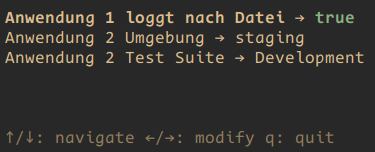
\includegraphics[scale=0.5]{post-start.png}}
    \end{center}
\end{figure}

\paragraph{Ansicht}
Abb. \ref{post-start} zeigt eine typische Ansicht direkt nach dem Start des
Programms. Die ersten drei Zeilen repräsentieren jeweils einen Eintrag in
der Konfigurationsdatei und somit eine Ziel-\gls{Textpassage} mit ihrem
aktuellen Wert. Jede dieser Zeilen besteht aus dem in der Konfigurationsdatei
vergebenen Titel des Eintrags, einem Pfeil und dem aktuellen Wert der Ziel-\gls{Textpassage}.
Die \textbf{aktuell ausgewählte Zeile} ist fett gedruckt während
\textcolor{teal}{der aktuelle Wert} blau dargestellt wird. Die genaue Darstellung
ist dabei vom verwendeten Terminal-Emulator und dessen Einstellungen bezüglich
Schriftart und Farbwerten abhängig.

\paragraph{}
Die ausgegraute Zeile am unteren Rand beschreibt in Kurzform die verfügbaren
Kommandos und die davon ausgelösten Aktionen.

\paragraph{Aktionen}
Die Hauptfunktionen werden über die vier Pfeiltasten gesteuert. Die Pfeiltasten
hoch bzw. runter bewegen die Zeilenmarkierung nach oben bzw. unten. Die Pfeiltasten
links bzw. rechts schalten den zur markierten Zeile gehörigen Wert weiter zum
nächsten Wert aus der konfigurierten Liste der möglichen Werte
(siehe Kapitel \ref{Konfiguration} - Konfiguration). Beim Umschalten eines Werts
wird die zugehörige Zieldatei entsprechend modifiziert.

\paragraph{} Mit einem Tastendruck auf q kann das Programm jederzeit beendet werden
und zur Kommandozeile zurückgekehrt werden.